% Project Specifications

\chapter{Implementation Details}

\section{Development Environment and Method}

Xilinx Vivado version 2017.04 is used as the development platform for \gls{fpga}. The typical workflow involves
the following steps:

\begin{itemize}
  \item Design the functionality of module and the I/O ports
  \item Implement the module in Verilog, add IP blocks if necessary
  \item Write the testbench for the module, run behavioral simulation to confirm the module behaves as
    expected
  \item Run synthesis and implementation
  \item View synthesis and implementation reports to see if there are any issues, especially with timing
  \item Create bitstream and test on device
\end{itemize}

    A parallel C implementation is developed on Linux simultaneously to facilitate the \gls{fpga} development.
Its main function is to provide algorithm verification, especially numerical comparison of output layers
    between software implementation and \gls{fpga} implementation.

\section{Implementing the Transposed Convolutional Layer}

The first step in implementing the transposed convolutional layer is to simulate the nested C loops
described in listing \ref{code:transposed_convolution_in_c}. For a for-loop shown in listing
\ref{code:simple_for_c}, the corresponding Verilog code is shown in listing \ref{code:simple_for_verilog}
% The module is modeled as a FSM.

\begin{code}
\begin{minted}{c}
for (int i = 0; i < m; i++) {
    for (int j = 0; j < n; j++) {
        // ...
    }
}
\end{minted}
  \captionof{listing}{Simple nested for-loop in C}
\label{code:simple_for_c}
\end{code}

\begin{code}
\begin{minted}{verilog}
reg [31:0] i = 0, i_next = 0;
reg [31:0] j = 0, j_next = 0;

always @(posedge clk)
begin
    i <= i_next;
    j <= j_next;
end

always @*
begin
    i_next = i;
    j_next = j;

    case (state)
        start:
            begin
                i_next = 0;
                j_next = 0;
                state_next = loop;
            end
        loop:
            begin
                if (j == n - 1)
                    begin
                        if (i == m - 1)
                            state_next = end;
                        i_next = i + 1;
                        j_next = 0;
                    end
                else
                    j_next = j + 1;
            end
        end:
            begin
            // finish the loop...
            end
        // handle other states ...
    endcase
end
\end{minted}
  \captionof{listing}{Simple for-loop in Verilog}
\label{code:simple_for_verilog}
\end{code}

The code is separated into a sequantial block and a combinational next-state logic block for clarity.
The merged C code of \mintinline{c}{gemm} and \mintinline{c}{col2im} shown in listing
\ref{code:transposed_convolution_in_c} can be then translated into Verilog using the structure
as a template.

The \mintinline{c}{transconv} module is connected to the input, weight, and output \glspl{bram}. A single
8-bit or 32-bit data is read or writtenin every cycle, which is quite inefficient. On the other hand,
although the data bus width can be configured for the \gls{bram}, a maximum of two read ports are available.
So it is possible to increase the data bus width to read more bytes in each cycle, but this is left
as a future work for optimization. Indeed, I/O is the main bottleneck in the design, as in many other systems.

The DSP48 Macro IP is utilized to accomplish computations with multiplication and accumulation. The first
block implements the operations shown in table \ref{table:dsp48_0_operations}. The second block is the core
MACC unit, and only contains $P \leftarrow A*B+P$.

\begin{table}[h]
  \centering
  \caption{DSP48 0 Operations}
  \begin{tabular}{l | l}
    0 & $P \leftarrow A*B-C$ \\
    1 & $P \leftarrow A*B+PCIN$ \\
    2 & $P \leftarrow A*B+C$
  \end{tabular}
  \label{table:dsp48_0_operations}
\end{table}

The ports of both blocks are shown in figure \ref{fig:dsp48_macro_0} and figure \ref{fig:dsp48_macro_1}.

\begin{figure}[h]
  \centering
  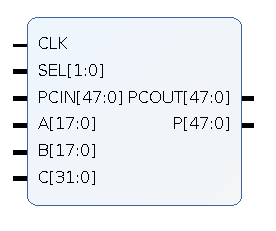
\includegraphics[scale=0.5]{dsp48_macro_0}
  \caption{DSP48 Macro 0 Ports}
  \label{fig:dsp48_macro_0}
\end{figure}

\begin{figure}[h]
  \centering
  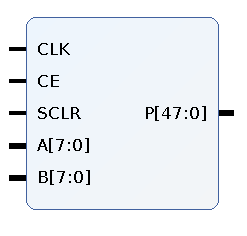
\includegraphics[scale=0.5]{dsp48_macro_1}
  \caption{DSP48 Macro 1 (MACC) Ports}
  \label{fig:dsp48_macro_1}
\end{figure}

\subsection{DSP48 Pipelining}

The DSP48 slice can be used without pipelining. However, that is essentially a combinational circuit and
the propagation delay will significantly reduce $F_{max}$. To run the \gls{fpga} at a higher frequency, it is
necessary to use pipeline registers. In our first design, only the register after the multiplier is used
therefore the result is delayed by one clock cycle.

\begin{figure}[h]
  \centering
  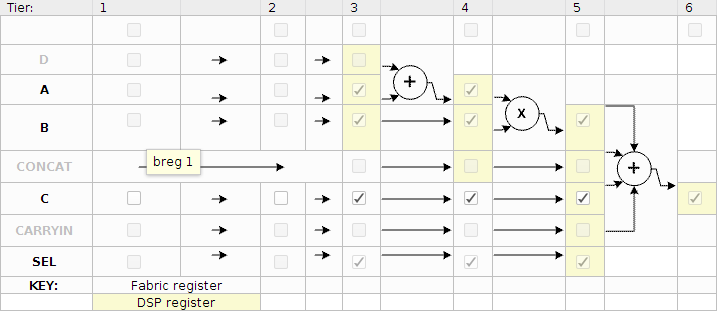
\includegraphics[scale=0.5]{dsp48_macro_0_pipeline}
  \caption{DSP48 Macro 0 Pipeline Configuration}
  \label{fig:dsp48_macro_0_pipeline}
\end{figure}

\section{Implementing the Other Layers}

The batch normalization layer, ReLU layer, and Tanh layer are implemented with floating-point numbers.
Xilinx Vivado is shipped with a Floating-point IP which supports many common operations, including
conversion between fixed-point and floating-point formats, multiplication, accumulation, exponential,
inverse square root, and many others. The input precision can be configured as half, single or
double-precision, or even customized width of exponent and fraction. It is also possible to choose
DSP slice usage, from logic only to maximum three DSP48 slices. Finally, the user is able to decide
the goal of optimization, using minimum resources or maximum clock frequency $F_{max}$. An example
floating-point multiplier is shown in figure \ref{fig:floating_point_multiplier}.

\begin{figure}[h]
  \centering
  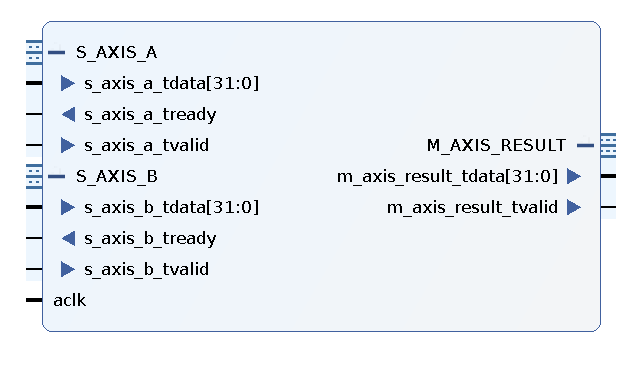
\includegraphics[scale=0.5]{floating_point_multiplier}
  \caption{A Configured Floating-point Multiplier IP Instance}
  \label{fig:floating_point_multiplier}
\end{figure}

\section{Testbench}

\begin{figure}[h]
  \centering
  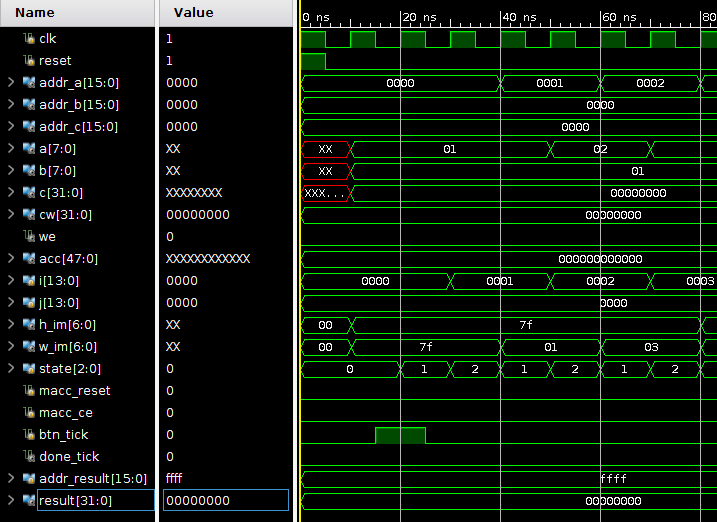
\includegraphics[scale=0.5]{behavioral_simulation}
  \caption{Behavioral Simulation of Transposed Convolution Module}
  \label{fig:behavioral_simulation}
\end{figure}

\section{Future Work on Optimization}

The first obvious optimization is to transfer all weight data from Dual-SPI Flash to the \gls{psram} once
the \gls{fpga} is configured. Weights will be loaded from the \gls{psram} subsequently, which has a parallel
interface and results in much faster loading of weights.

The second optimization is to further introduce several small caches using distributed RAM. These caches
are implemented using \glspl{lut} and are faster than \glspl{bram}, i.e., they can be read asynchronously.
Once inputs and weights are loaded into these caches, computation can then be carried out in parallel,
making use of more DSP48 slices.

\clearpage %force the next chapter to start on a new page. Keep that as the last line of your chapter!
